\chapter{Analyse mit CryptoMiniSat}
\label{chp:analyse}

mehrere durchläufe mit cryptominisat\\
ein durchlauf besteht aus mehreren lösungsversuchen mit jeweils einem bit vorgabe mehr\\
reale werte nur per assumptions, um allgemeine klauseln zu erhalten\\
bei jeder lösung werden klauseln rausgeschrieben\\
kein unterschied zwischen redundant und irredundant - beides wird analysiert\\
statistiken aus sql einfügen: anteil der klauseln länge x an propagation und wieviele literale konnten festgelegt werden\\
im folgenden die schritte der analyse:

\section{Aussortieren bekannter und doppelter Klauseln}

\TODO{erledigen}

ganz einfach. kein wissensgewinn\\
c++ set\\
bekanntes aussortieren um ermitteltes wissen zu gewinnen\\
bekannt ist die kombination aus mit und ohne xor
\section{Erkennen und normalisieren modulspezifischer Klauseln}
\label{sec:ana:module}

Nach dem Aussortieren der schon bekannten Klauseln werden die neuen Klauseln den einzelnen Modulen zugeordnet. Durch die hierarchische Anordnung
muss beachtet werden, dass eine Klausel mehreren Modulen zugeordnet werden kann. Sinnvoll ist es jedoch, die Klausel nur dem Modul zuzuordnen
das in der Hierarchie möglichst weit unten steht. Wird eine Klausel für einen Addierer gefunden, kann diese Klausel so zukünftig für alle Addierer
genutzt werden, während sie im Modul für die vollständige Kompressionsfunktion nur für den einen speziellen Addierer gelten würde. Um diese
Zuordnung zu realisieren erhält jedes Modul ein Level. Im hierarchischen Aufbau muss das Level eines Moduls dabei höher sein, als das höchste Level
der verwendeten Module. Die vergebenen Level sind in Abbildung \ref{fig:sha256_module_level} dargestellt.
\begin{figure}[!h]
  \centering
  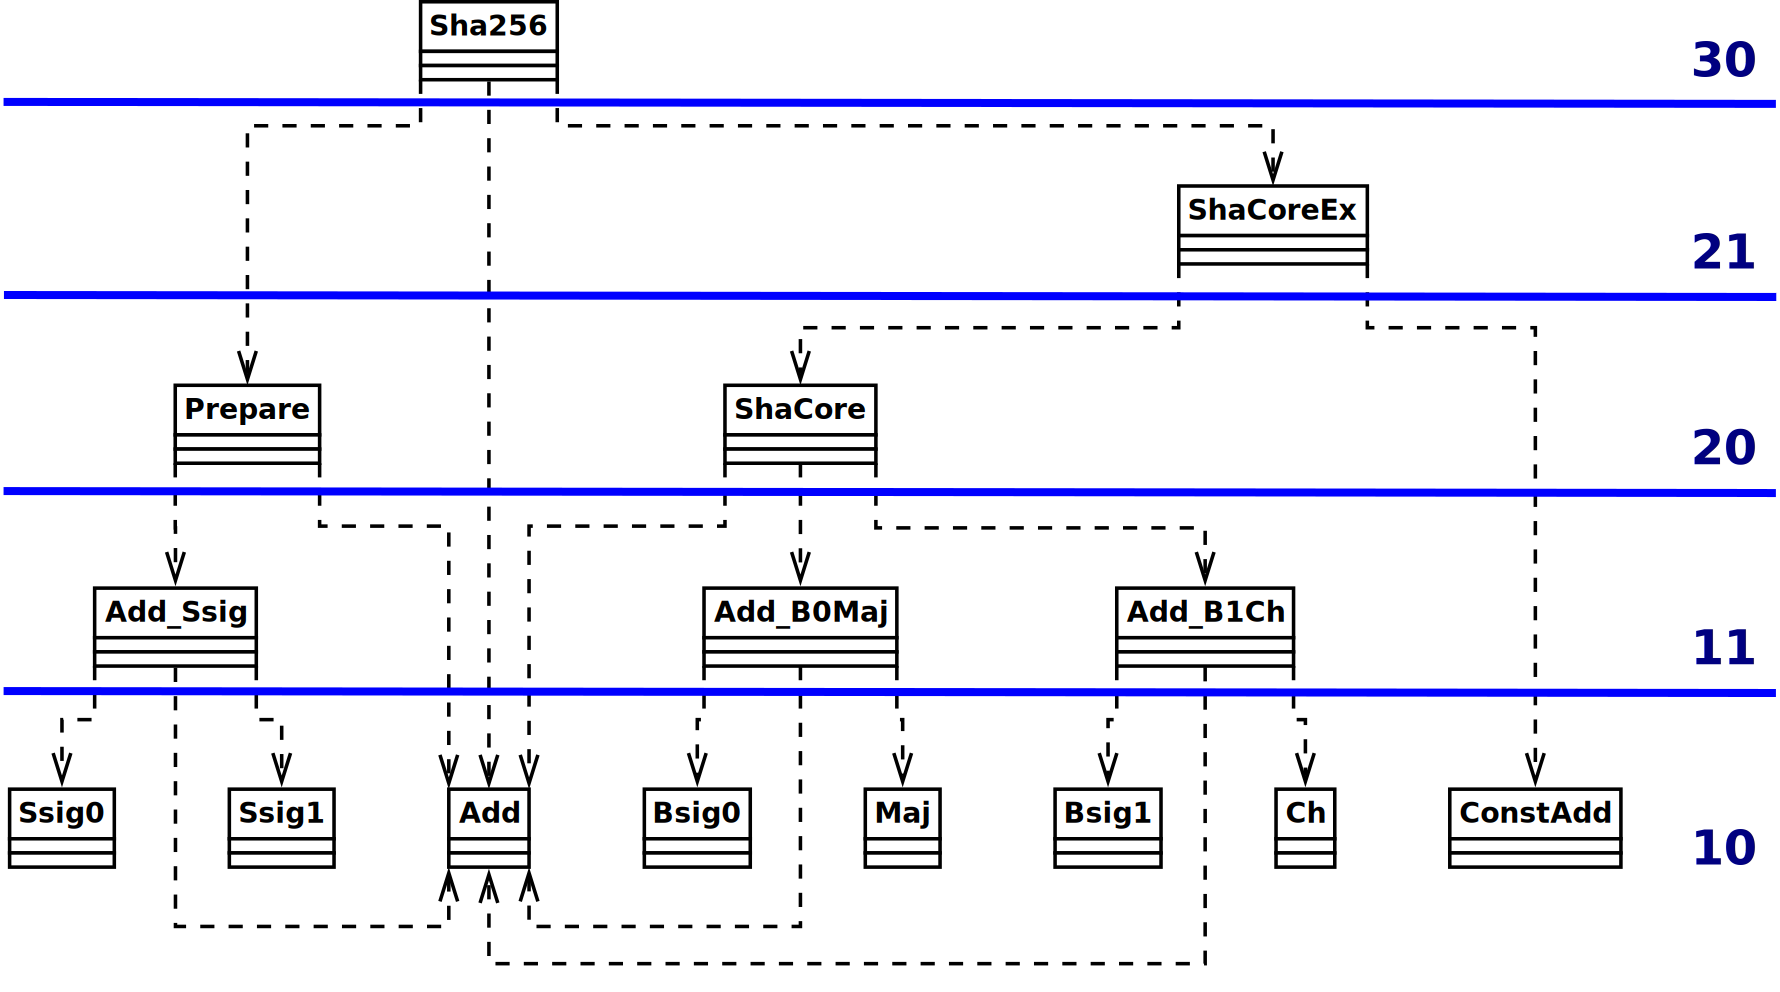
\includegraphics[scale=0.265]{images/module_level}
  \caption{Modullevel von \glos{sha256}}
  \label{fig:sha256_module_level}
\end{figure}

Die Level werden nicht fortlaufend nummeriert, um bei Bedarf weitere Module/Level einfügen zu können, ohne die Level der vorhandenen Module anpassen zu müssen.

Anhand der Level können die Module sortiert werden, so dass die Prüfung, ob eine Klausel zum Modul gehört, bei den Modulen mit dem niedrigsten Level beginnen kann.
Eine Klausel gehört dann zu einem Modul, wenn alle Literale der Klausel im Modul verwendet werden. Dabei kann es sich um Eingänge, zusätzliche Literale oder Ausgänge
handeln. Ein Sonderfall ist eine Klausel die ausschließlich aus Eingangsliteralen oder ausschließlich aus Ausgangsliteralen besteht. Die Ausgangsliterale eines Moduls
sind im allgemeinen die Eingangsliterale eines anderen Moduls wodurch die Zuordnung bei gleichem Level unklar ist. Klauseln dieser Art wurden bei der Analyse jedoch
nicht gefunden. 

Für die Zuordnung der Klauseln wird zunächst ein Collector mit dem Namen "`ModulDB"' implementiert. Die ModulDB überschreibt nur die Methode newModul des Collectors,
um die Registrierung der Module zu erfassen. Generierte Klauseln, die an die Methode create übergeben werden, werden dadurch ignoriert. Erfasst werden neben dem
Modulnamen und dem Level die verwendeten Literale in der Reihenfolge: Eingänge, zusätzliche Literale und Ausgänge. ModulDB stellt außerdem eine Funktion bereit,
der eine beliebige Klausel zur Zuordnung übergeben werden kann. Wird ein passendes Modul gefunden, wird ein Zeiger auf die Modulinformationen zurückgeliefert.

Das Programm "`modulchecker"' nutzt schließlich die ModulDB für die Zuordnung. Zunächst wird ein Objekt der Kompressionsfunktion erzeugt, in das die ModulDB als
Besucher übergeben wird. Danach werden die im vorigen Abschnitt erstellten DIMACS-Dateien eingelesen und jede Klausel einem Modul zugeordnet. Die Zuordnung wird
in diesem Fall immer gelingen, da spätestens die Kompressionsfunktion alle Literale umfasst.

Da die Module in ihrer Normalform implementiert werden (siehe Kapitel \ref{chp:knf}) kann eine zugeordnete Klausel noch nicht direkt genutzt werden.
Die verwendeten Literale in der Kompressionsfunktion sind andere als die des Moduls in der Normalform. Wird eine Klausel zugeordnet, erfolgt deshalb
direkt im Anschluss die Normalisierung der Klausel. Diese wird auf Basis der im Modul verwendeten Literale durchgeführt. Da diese in der richtigen
Reihenfolge vorliegen, können in der Klausel vorkommende Literale darin erkannt und anhand des Index in das Literal der Normalform überführt werden.

Nach der Normalisierung werden die Klauseln für jedes Modul in einem eigenen "`set"' gesammelt. Wie in Abschnitt \ref{sec:ana:rem_double} erfolgt
dadurch automatisch aussortierung doppel \TODO{hmm}.

mehrfach erkannt - set - wird aussortiert.


Programm "`clausechecker"' : testen der klauseln : vielleicht ungültig.


\begin{figure}[!h]
  \centering
  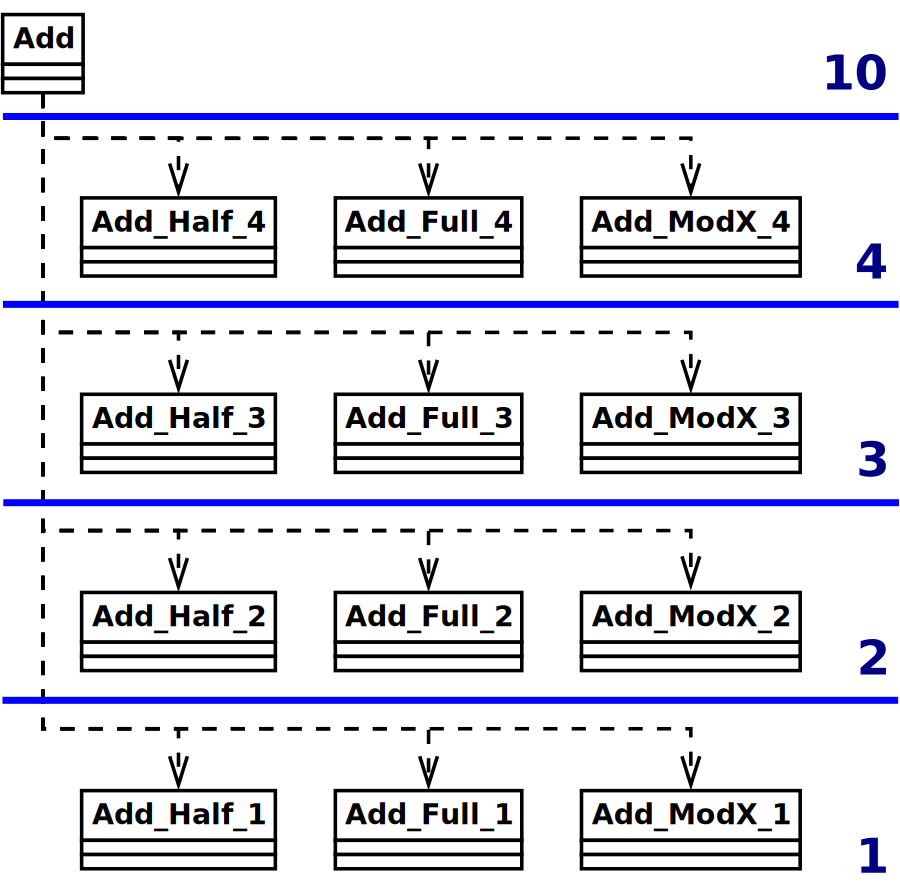
\includegraphics[scale=0.265]{images/module_add}
  \caption{Ergänzte Module von \glos{sha256}}
  \label{fig:sha256_module_add}
\end{figure}


\TODO{erledigen}


\section{Distanzermittlung von Klauseln in der Kompressionsfunktion}
\label{sec:ana:distance}

Die Analyse der neuen Klauseln aus der Kompressionsfunktion erfolgt auf Basis einer Distanzmetrik. Je höher die Distanz einer Klausel, desto höher
ist ihr angenommener Wert. Eine hohe Distanz bedeutet, dass die Klausel Literale aus Modulen in Zusammenhang bringt, die bisher in keiner direkten
Beziehung stehen.

Für die Distanzberechnung wird ein ungerichteter Graph aus den Modulen mit Level zehn erstellt. Ein Modul definiert sich dabei aus zusätzliche Literalen
und den Ausgangsliteralen. Im Gegensatz zum letzten Abschnitt fallen die Eingangsliterale weg, um eine eindeutige Zuordnung eines Literals zu einem
Modul durchführen zu können. Realisiert wird der Graph durch einen Collector mit dem Namen "`ModulGraph"'. Genau wie die ModulDB aus dem letzten Abschnitt
überschreibt der ModulGraph nur die Methode newModul des Collectors, um die Registrierung der Module zu erfassen. Um die Zuordnung der Literale zu einem
Modul schnellstmöglich durchführen zu können, wird eine Lookup-Tabelle erstellt, in der zu jedem Literal das zugehörige Modul hinterlegt ist. Registriert
sich ein Modul im ModulGraph, erfolgt zunächst die Aufnahme in die Lookup-Tabelle. Direkt im Anschluss wird das Modul mit den Modulen verknüpft, die die
Eingangswerte liefern, und so der ungerichtete Graph erstellt.

Der ModulGraph stellt eine Funktion "`printGraph"' bereit, mit der der ungerichtete Graph visualisiert werden kann. Die Ausgabe erfolgt in der Sprache DOT \cite{lang:dot}
mit der Graphen einfach beschrieben werden können. Mit Hilfe eines Renderes kann die Beschreibung des Graphen in ein Grafikformat überführt werden.
Optional kann als Parameter eine Klausel übergeben werden um Module, deren Literale in der Klausel vorkommen, farblich hervorzuheben. Abbildung \ref{fig:sha256_graph}
zeigt einen Ausschnitt aus dem vollständigen Graphen der Kompressionsfunktion. Abgebildet ist die dritte Anwendung der Rundenfunktion. Neben den
Modulnamen werden die verwendeten Literale ausgegeben. Da der Addierer zusätzliche Literale benötigt (Carrybits), sind bei diesem zwei Bereiche aufgeführt.
Die anderen Module kommen ohne zusätzliche Literale aus und enthalten somit nur die Ausgangsliterale. Anzumerken sind die fünf ausgehenden Kanten der beiden
finalen Addierer der Rundenfunktion. Die Ergebnisse werden jeweils in den vier folgenden Runden in fünf weiteren Modulen verwendet.
\begin{figure}[!h]
  \centering
  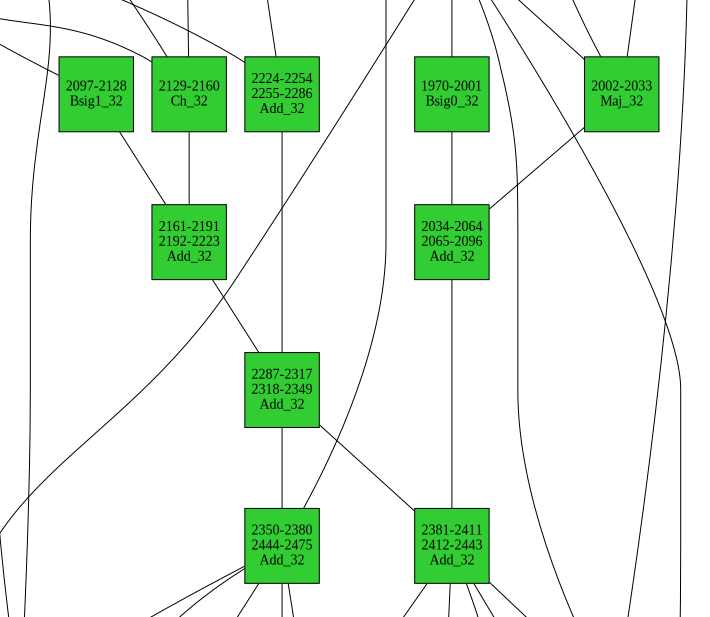
\includegraphics[scale=0.43]{images/sha256graph}
  \caption{Ausschnitt des ungerichteten Graphen von \glos{sha256}}
  \label{fig:sha256_graph}
\end{figure}

Nach der Erstellung des Graphs werden die Distanzen der Module untereinander berechnet. Für jedes Modul wird dafür der Dijkstra-Algorithmus \cite{dijkstra} angewandt,
um die Distanzen zu allen anderen Modulen zu berechnen. Jede Kante bekommt dabei das Gewicht eins. Genau wie für die Zuordnung der Literale zu den Modulen wird für
die Distanzermittlung eine Lookup-Tabelle verwendet. In jedem Knoten werden so die Distanzen zu allen anderen Modulen abgelegt. Für die vollständige Kompressionsfunktion
von \glos{sha256} stellt sich heraus, dass die größte Distanz zwischen zwei Modulen sechzehn beträgt; Es liegen somit maximal fünfzehn Module zwischen zwei anderen
Modulen. Berechnet werden durch den Dijkstra-Algorithmus auch die Wege für die die Distanz gilt. Die Wege haben jedoch für diese Arbeit keine Relevanz und werden
verworfen. Durch die Lookup-Tabellen kann die Berechnung der Distanzen einmalig bei Programmstart erledigt werden und große Klauselmengen können effizient bewertet werden.

Nachdem die Distanzen der einzelnen Module bekannt sind, kann damit die Distanz einer Klausel berechnet werden. Da eine Klausel mehr als zwei Module betreffen kann, werden
die Distanzen aller betroffenen Module überprüft und die größte Distanz ausgewählt. Ermittelt wird außerdem die Anzahl der betroffenen Module. Ein Klausel mit sechs Literalen
kann zum Beispiel zwei Module betreffen, wenn je drei Literale aus einem Modul stammen. Die Distanz einer Klausel ergibt sich aus der Formel in Abbildung \ref{eq:clausedistance}.
\begin{figure}[!h]
  \begin{align*}
  Klauseldistanz = gr\ddot{o}{\beta}te~Moduldistanz - Modulanzahl + 1
  \end{align*}
  \caption{Formel zur Berechnung der Distanz einer Klausel}
  \label{eq:clausedistance}
\end{figure}

Die Formel soll anhand eines Beispiels erläutert werden bei dem eine Klausel mit vier Literalen herangezogen wird. Die Zuordnung der Literale
zu den Modulen ergibt drei unterschiedliche Module. Bei dem Vergleich der Distanzen zwischen den Modulen wird eine maximale Distanz von drei ermittelt.
Mit der Formel aus Abbildung \ref{eq:clausedistance} ergibt sich eine Klauseldistanz von eins.

Abbildung \ref{fig:distance} zeigt zwei mögliche Fälle, die dem Beispiel entsprechen. In den gezeigten Graphen sind die Module, denen mindestens ein Literal
zugeordnet wurde rot eingefärbt. Weitere Module denen kein Literal der Klausel zugeordnet werden konnte, sind in grün dargestellt.
\begin{figure}[!h]
  \centering
  \begin{minipage}[b]{6cm}
    \centering
    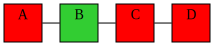
\includegraphics[scale=0.6]{images/distance1}\\
    Schlechtester Fall
  \end{minipage}
  \begin{minipage}[b]{6cm}
    \centering
    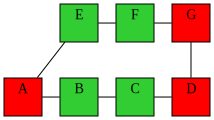
\includegraphics[scale=0.6]{images/distance2}\\
    Weiterer Fall
  \end{minipage}
  \caption{Beispiel für die Distanz einer Klausel}
  \label{fig:distance}
\end{figure}

Im schlechtesten Fall ergibt sich die maximale Distanz zwischen den Modulen A und D, wobei das dritte Modul C auf dem Pfad zwischen den Modulen A und D liegt.
Genau ein Modul B wird dabei übersprungen, was genau dem Wert der Klauseldistanz entspricht. Die Klauseldistanz sagt damit aus, wie viele Module im schlechtesten
Fall übersprungen werden.

Ein weiterer Fall zeigt, dass die Klauseldistanz auch höher sein kann, wenn weitere Pfade von Modul A nach Modul D führen. Ein weiterer Pfad ist jedoch mindestens
genau so lang wie der erste Pfad. Angenommen der zusätzliche Pfad hat die Länge vier und das dritte betroffenen Modul (in diesem Fall G) liegt auf diesem längeren
Pfad, werden zwei Module übersprungen.

Um die Distanz für die neuen Klauseln aus der Kompressionsfunktion zu ermitteln, wird das Programm "`distancechecker"' erstellt. Dieses Programm liest alle Klauseln
ein und verteilt diese je nach Klauseldistanz auf eine eigene DIMACS-Datei. Vernachlässigt wird bei diesem Vorgehen die Länge der Klausel. Die Anzahl der Literale
wird nur indirekt durch die Anzahl der betroffenen Module berücksichtigt. Dies wird aber vernachlässigt, da Klauseln mit großer Länge und Distanz durchaus interessant
sein könnten, auch wenn es eher unwahrscheinlich ist, dass sie den Lösungsprozess in CryptoMiniSat beschleunigen.

Bei der Analyse zeigt sich, dass die Distanz der Klauseln breit gestreut ist. Die Distanz reicht von $5$ bis unter $-250$. Wird zum Vergleich eine Klausel betrachtet,
die einem einzelnen Modul mit Level zehn zugeordnet ist, ergibt sich dafür eine Klauseldistanz von $0$ ($= 0 - 1 + 1$). Darauf basierend werden im weiteren Verlauf
nur Klauseln berücksichtigt, deren Distanz größer als null ist, in der Erwartung, dass sie zusätzliches Wissen darstellen und den Lösungsprozess beschleunigen.
\section{Prüfung auf kürzere vorhandene Klauseln}
\label{sec:ana:sub}

\TODO{erledigen}
\section{Auflistung gelernter Klauseln}

\TODO{erledigen}